% !TEX root = ./article.tex

\documentclass{article}

\usepackage{mystyle}
\usepackage{myvars}



%-----------------------------

\begin{document}

	\maketitle % Insert title

	\thispagestyle{fancy} % All pages have headers and footers


%-----------------------------
%	ABSTRACT
%-----------------------------

	\begin{abstract}
		\noindent [TODO ]
	\end{abstract}

%-----------------------------
%	TEXT
%-----------------------------


	\section{Introducción}
	\label{sec:introducción}

		\paragraph{}
		[TODO]

	\section{La figura \ref{e1:plot} muestra un conjunto de entrenamiento con ejemplos positivos (estrellas) y negativos (círculos). Se desea clasificar la nueva instancia $<3,3>$ mediante el algoritmo $K$-vecinos más próximos. Obtener la clasificación para los valores de $K=\{ 1, 3, 5\}$ utilizando las distancias indicadas a continuación}
	\label{sec:e1}

		\paragraph{}
		[TODO]

		\begin{figure}[h]
			\begin{center}
				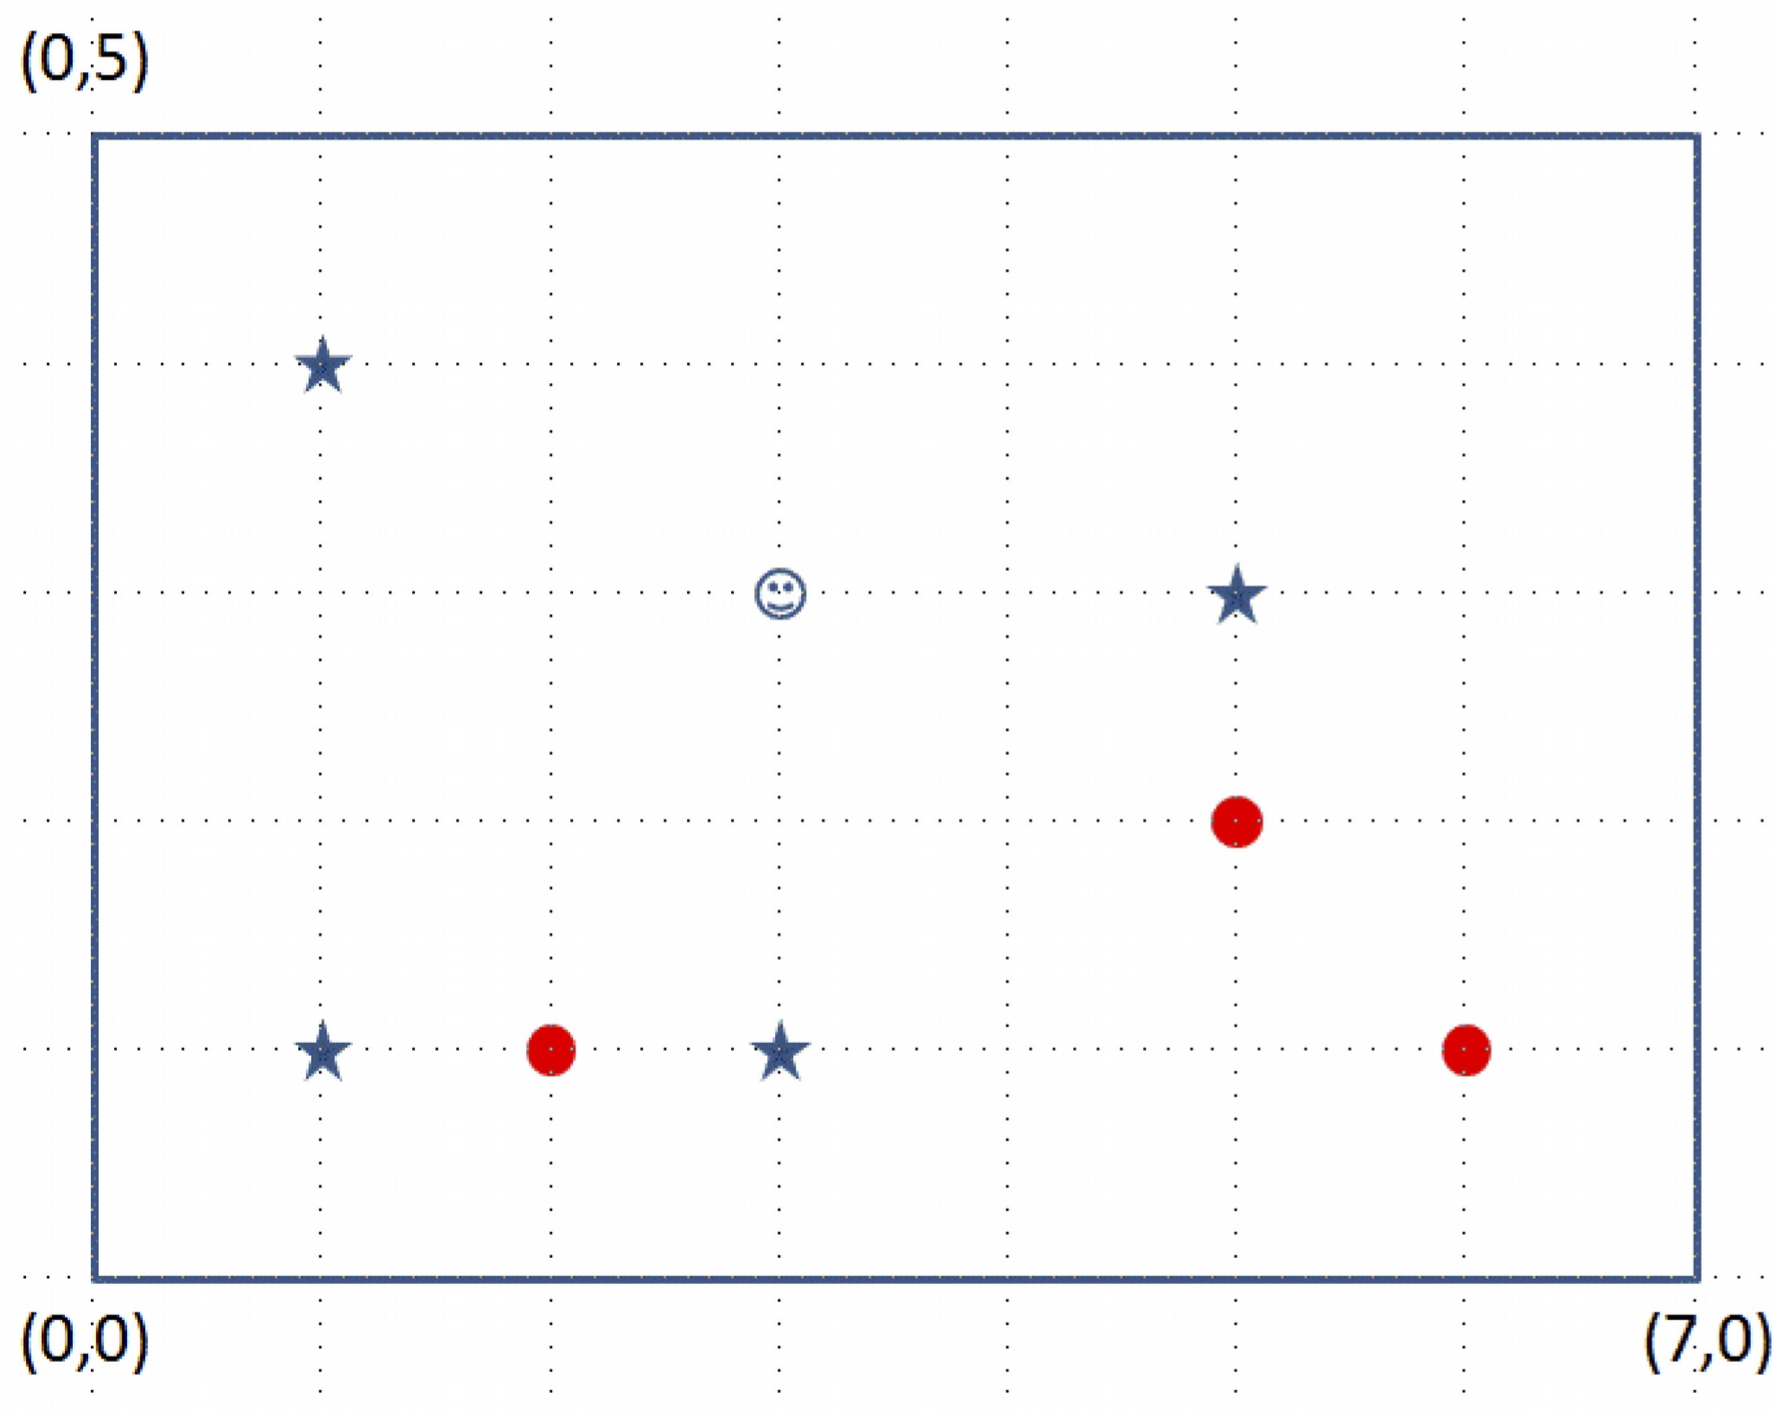
\includegraphics[width=0.5\textwidth]{exercise-1-plot}
			\end{center}
			\caption{Representación Gráfica del problema \ref{sec:e1}}
			\label{e1:plot}
		\end{figure}

		\subsection{Distancia Euclídea}

			\paragraph{}
			[TODO]

		\subsection{Distancia Euclídea Ponderada: $w_x=0.2, w_y=0.8$}

			\paragraph{}
			[TODO]

		\subsection{Distancia de Manhattan}

			\paragraph{}
			[TODO]

		\subsection{Distancia de Hamming}

			\paragraph{}
			[TODO]

	\section{Dígitos manuscritos}

		\paragraph{}
		[TODO]


%-----------------------------
%	Bibliographic references
%-----------------------------
	\nocite{garciparedes:machine-learning-instance-based}
	\nocite{subject:taa}
	\nocite{tool:weka}
  \bibliographystyle{alpha}
  \bibliography{bib/misc}

\end{document}
